\usetikzlibrary{shapes,arrows,fit,calc,positioning}
\usetikzlibrary{backgrounds}
\tikzstyle{box} = [draw, rectangle, fill=white, rounded corners, thick, node distance=7em, text width=10em, text centered, minimum height=3.5em]
\tikzstyle{container} = [draw, rectangle, dashed, inner sep=2em]
\tikzstyle{line} = [draw, thick, -latex']

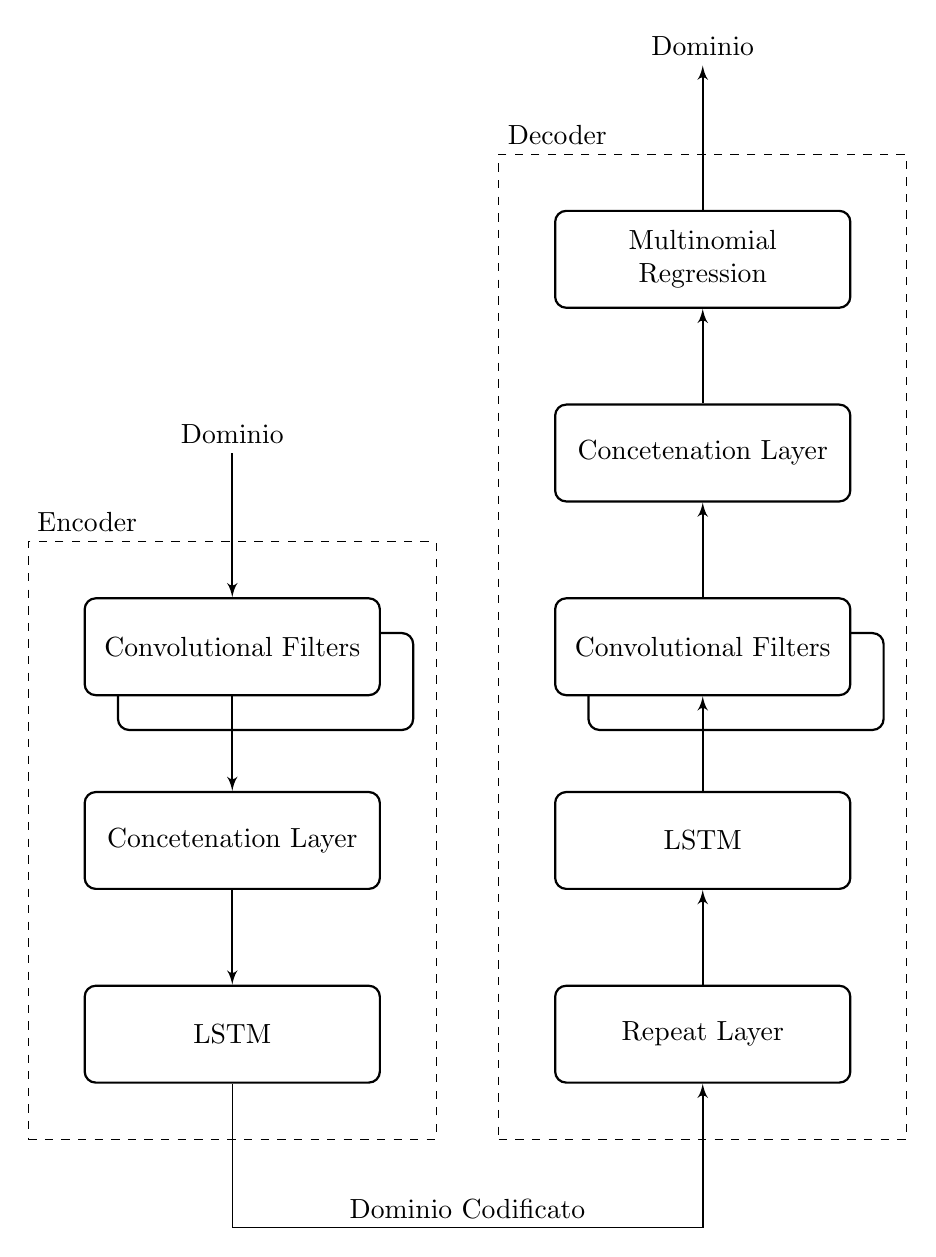
\begin{tikzpicture}[auto]
    \node [box] (cnn) {Convolutional Filters};
    \coordinate[above of=cnn, node distance=7em](begin_enc);
    \node at (begin_enc.north) [above,node distance=0 and 0] {Dominio};
    \node [box, below of=cnn] (conc) {Concetenation Layer};
    \begin{scope}[on background layer]
   		 \node [box,above left=-17mm and -42mm of cnn ] (note1){ };
   	\end{scope}
    \node [box, below of=conc] (LSTM) {LSTM};
	\coordinate[below of=LSTM,node distance=7em](end_enc);
    
    \node [box, right of=LSTM, node distance=17em] (rep) {Repeat Layer};
   	\coordinate[below of=rep, node distance=7em](begin_dec);    
    \node [box, above of=rep] (LSTM2) {LSTM};
    \node [box, above of=LSTM2] (cnn2) {Convolutional Filters};
    \begin{scope}[on background layer]
   		 \node [box,above left=-17mm and -42mm of cnn2 ] (note1){ };
   	\end{scope}
	\node [box, above of=cnn2] (conc2) {Concetenation Layer};
	\node [box, above of=conc2] (dense) {Multinomial Regression};
	\coordinate[above of=dense, node distance=7em](end_dec);
    \node at (end_dec.north) [above,node distance=0 and 0] {Dominio};

    %\coordinate (middle) at ($(resources.east)!0.5!(sensors.east)$);
    %\node [box, left of=middle, node distance=10em] (archive) {Archive};
    %\node [box, left of=archive, node distance=10em] (reporting) {Reporting};
    \node[container, fit=(cnn) (LSTM)] (encoder) {};
    \node[container, fit=(dense) (rep)] (decoder) {};
    \node at (encoder.north west) [above right,node distance=0 and 0] {Encoder};
  	\node at (decoder.north west) [above right,node distance=0 and 0] {Decoder};

    %\node[container, fit=(archive) (reporting)] (his) {};
    %\node at (his.north west) [above right,node distance=0 and 0] {HIS};
	\path [line] (begin_enc) -- (cnn);
    \path [line] (cnn) -- (conc);
    \path [line] (conc) -- (LSTM);
    
    \path [line] (rep) -- (LSTM2);
	\path [line] (LSTM2) -- (cnn2);
	\path [line] (cnn2) -- (conc2);
	\path [line] (conc2) -- (dense);
	\path [line] (dense) -- (end_dec);
    
        
    \draw (LSTM) -- (end_enc);
    \path (end_enc) -- (begin_dec) node[midway] {Dominio Codificato};
    \draw (end_enc) -- (begin_dec);
    \draw [line] (begin_dec) -- (rep);

    %\path [line] (archive) |- (planning);
    %\path [line] (archive) |- (processing);
    %\path [line] (processing) -| (reporting);

    %\draw [line] (processing.east) -- ++(2,0) node(lowerright){} |- (planning.east);
    %\draw [line] (lowerright |- or.east) -- (or.east -| resources.south east);
\end{tikzpicture}
